\documentclass[journal]{IEEEtran}
% IEEE Transactions on Industrial Informatics -- anonymous regular-paper draft
% Compile: latexmk -pdf main.tex
\usepackage{amsmath,amssymb,amsfonts}
\usepackage{algpseudocode}
% Local XeTeX/Tectonic builds: route IEEEtran's ptm (Times) family requests to
% the legacy Times Type1 faces so metrics match the pdfLaTeX reference build;
% the latexmk -pdf (pdfLaTeX) path is unaffected.
\usepackage{iftex}
\ifxetex
  \DeclareFontFamily{TU}{ptm}{}
  \DeclareFontShape{TU}{ptm}{m}{n}{<->ptmr8t}{}
  \DeclareFontShape{TU}{ptm}{b}{n}{<->ptmb8t}{}
  \DeclareFontShape{TU}{ptm}{m}{it}{<->ptmri8t}{}
  \DeclareFontShape{TU}{ptm}{b}{it}{<->ptmbi8t}{}
  \DeclareFontShape{TU}{ptm}{m}{sl}{<->ptmro8t}{}
  \DeclareFontShape{TU}{ptm}{m}{sc}{<->ptmr8t}{}
\fi
\usepackage{graphicx}
\usepackage{booktabs}
\usepackage{tabularx}
\usepackage{array}
\usepackage[table]{xcolor}
\usepackage{stfloats}
\usepackage{placeins}
\usepackage{url}
\urlstyle{same}
% Cross-references and citations. The cite package renders IEEE-style citation
% groups ([14]--[16], [20], [21]) with hyperref support.
\usepackage{cite}
\usepackage[colorlinks=true,linkcolor=black,citecolor=black,urlcolor=black]{hyperref}
\hypersetup{bookmarksnumbered=true,
  pdftitle={AgentWorkShop: A Configurable Framework for Multi-Scenario Industrial Agent Integration},
  pdfauthor={},
  pdfsubject={IEEE Transactions on Industrial Informatics},
  pdfkeywords={industrial informatics, industrial agents, multi-agent systems, production system integration, semantic data integration}}

% Float placement only; IEEEtran margins and body type remain unchanged.
\setcounter{topnumber}{4}
\setcounter{bottomnumber}{3}
\setcounter{totalnumber}{7}
\setcounter{dbltopnumber}{1}
\renewcommand{\topfraction}{0.95}
\renewcommand{\bottomfraction}{0.80}
\renewcommand{\textfraction}{0.03}
\renewcommand{\floatpagefraction}{0.72}
\renewcommand{\dbltopfraction}{0.95}
\renewcommand{\dblfloatpagefraction}{0.72}

% Tight but conventional float separation; body type and margins are unchanged.
\setlength{\textfloatsep}{8pt plus 2pt minus 3pt}
\setlength{\dbltextfloatsep}{8pt plus 2pt minus 3pt}
\setlength{\intextsep}{7pt plus 2pt minus 3pt}
\setlength{\abovecaptionskip}{3pt plus 1pt minus 1pt}
\setlength{\belowcaptionskip}{2pt plus 1pt minus 1pt}

% Evidence snapshot: one archived integrated run with raw reports, run
% manifest, scenario definitions, and metrics.
% The two live engine-task logs are original outputs saved at execution time,
% as confirmed by the author; the structured run report retains their checked
% outcomes. The four-arm ablation has its own companion run record.
\newcommand{\resSeed}{42}
\newcommand{\resPhases}{20}
\newcommand{\resChecksTotal}{83}
\newcommand{\resChecksPass}{83}
\newcommand{\resChecksWarn}{0}
\newcommand{\resChecksFail}{0}
\newcommand{\resTotalWall}{26\,min}
\newcommand{\resDaqSamples}{55}
\newcommand{\resWriteP}{29.954\,ms}
\newcommand{\resTcpP}{47.8\,ms}
\newcommand{\resOpcP}{19.8\,ms}
\newcommand{\resMqttP}{19.3\,ms}
\newcommand{\resHttpP}{32.9\,ms}
% p95 per protocol line, same run: ~6 writes each. Recorded in the archive's
% metrics.csv (write_p95_ms) but reported in the body only since the 2026-10-12
% revision, so they live here rather than inline. Names must be letters only:
% \resTcpP95 would parse as \resTcpP followed by the characters "95".
\newcommand{\resTcpTail}{248.9\,ms}
\newcommand{\resOpcTail}{20.5\,ms}
\newcommand{\resMqttTail}{20.1\,ms}
\newcommand{\resHttpTail}{44.6\,ms}
% cross-protocol ranges over the four write families (min p50 = MQTT, max
% p50 = Modbus TCP; min p95 = MQTT, max p95 = Modbus TCP)
\newcommand{\resPfiftyRange}{19.3--47.8\,ms}
\newcommand{\resPninetyfiveRange}{20.1--248.9\,ms}
\newcommand{\resWriteNperLine}{6}
\newcommand{\resAblationRun}{\texttt{20260921181234-e1lite}}
\newcommand{\resFullIntercept}{18/18}
\newcommand{\resNoInterlockIntercept}{12/18}
\newcommand{\resNoReadbackIntercept}{18/18}
\newcommand{\resUngatedIntercept}{12/18}
\newcommand{\resBackstop}{130.2\,s}
% 134.7 s: defined but NOT used in the body (the drill's archived timing is
% 130.196 s, = \resBackstop); kept only so the symbol is not silently reused.
\newcommand{\resBackstopDrill}{134.7\,s}
\newcommand{\resPortFfive}{9/9}
\newcommand{\resPortCode}{0}
\newcommand{\resParamChecks}{4/4}
\newcommand{\resHitlLatency}{461\,ms}
\newcommand{\resMissionFrom}{200}
\newcommand{\resMissionTo}{204.704}
\newcommand{\resMissionPv}{204.70}
\newcommand{\resMissionTarget}{$204.704\pm0.75$}
\newcommand{\resBiaxSp}{30}
\newcommand{\resBiaxDaq}{19}
\newcommand{\resBiaxWrites}{3}
\newcommand{\resBiaxStart}{28.10}
\newcommand{\resBiaxFinal}{25.66}
\newcommand{\resBiaxTarget}{25.0}
\newcommand{\resBiaxTol}{0.7}
\newcommand{\resLlmWall}{156.3\,s}
\newcommand{\resGoalWall}{637.3\,s}
\newcommand{\resGoalFinal}{51.7}
\newcommand{\resJstar}{89.894}
\newcommand{\resJzero}{67.2}
\newcommand{\resControllerMin}{0.965}
\newcommand{\resControllerMean}{0.969}
\newcommand{\resControllerMax}{0.972}
\newcommand{\resInjStart}{31.25}
\newcommand{\resInjFinal}{32.17}
\newcommand{\resInjWrites}{2}
\newcommand{\resInjWall}{26.48\,s}
\newcommand{\resWwtpStart}{0.21}
\newcommand{\resWwtpFinal}{3.50}
\newcommand{\resWwtpWrites}{15}
\newcommand{\resWwtpWall}{169.27\,s}
\newcommand{\resWwtpCostStart}{181.5}
\newcommand{\resWwtpCostFinal}{179.1}
\newcommand{\resAnnealStart}{134.52}
\newcommand{\resAnnealFinal}{100.08}
\newcommand{\resAnnealWrites}{5}
\newcommand{\resAnnealWall}{102.76\,s}
\newcommand{\resAnnealSpeedFinal}{164}
\newcommand{\resAnnealSpeedTried}{176}
\newcommand{\resAnnealGain}{17.1\%}
% writeLockSeconds: node field default 30 s, constructor default 60 s; the
% online path enforces max(60 s, configured), so 60 s is the effective floor
% (unused in body since the pacing-window rewrite; kept for reference).
\newcommand{\resWriteLock}{60\,s}

% October 2026 deployment-scale campaign (v0.7.57), added with the revision.
% The hardened-pipeline run is archived at 91/91; three consecutive
% full-suite runs score 79/79 each (237 total; an earlier 80-per-run tally
% counted one S7 report assertion that is not a logged check). Per-run
% reports, manifests, and timelines are archived with each benchmark run.
\newcommand{\resPipeRun}{\texttt{benchmark-20261008045434}}
\newcommand{\resPipeTotal}{91}
\newcommand{\resPipeApi}{54}
\newcommand{\resCampaignRuns}{three consecutive}
\newcommand{\resCampaignTotal}{237}
\newcommand{\resCampaignApi}{45}
\newcommand{\resLoopTotal}{53}
\newcommand{\resAckTotal}{34}
\newcommand{\resDocsTotal}{91}
\newcommand{\resLinesLive}{34}
\newcommand{\resLinesRunning}{17}
% channel count across the three October 9 regression runs: 111/111/113;
% the body reports the range rather than one run's value.
\newcommand{\resChannelsLive}{111--113}
\newcommand{\resDaqOnline}{67}
\newcommand{\resWriteNodesLive}{77}
\newcommand{\resRecipesLive}{52}
\newcommand{\resBindingsLive}{385}
% approval->dispatch spans both campaigns: 8/9/9 ms (Oct 7-8), 9/6/6 ms (Oct 9).
\newcommand{\resHitlDispatchMs}{6--9\,ms}
\newcommand{\resLadderFrom}{66}
\newcommand{\resLadderTo}{63}
\newcommand{\resConsistencyErr}{0.0\,bar}
\newcommand{\resObsVerifyFast}{25.1\,s}
% 245.204 s (benchmark-20261007194413) / 245.184 s (-07194925), exact values
\newcommand{\resObsVerifyCadence}{245.20/245.18\,s}
\newcommand{\resCadenceWait}{218\,s}
\newcommand{\resWideRows}{869}

% October 9, 2026 regression campaign (v0.7.57), same live instance.
% Three runs archived at 92/92, 90/90, and 90/90; timeline.jsonl per run
% (S4/S5 process records, HITL card events).
\newcommand{\resNovRuns}{\texttt{benchmark-20261009021149}/\texttt{-024141}/\texttt{-033810}}
\newcommand{\resNovTotal}{272}
\newcommand{\resNovApi}{54}
\newcommand{\resNovDeadband}{0.15\,g}
\newcommand{\resNovZigzagFrom}{64}
\newcommand{\resNovZigzagTo}{63}
\newcommand{\resNovCorrFrom}{63}
\newcommand{\resNovCorrTo}{65}
\newcommand{\resNovWeights}{$32.49/32.33/32.22$\,g}
\newcommand{\resNovCadenceReject}{69\,s}
\newcommand{\resNovCardId}{\texttt{ap-2950a5b6}}
\newcommand{\resNovRunId}{\texttt{rr-51b0a0ac}}
\newcommand{\resNovScheme}{hold-pressure micro-up (sensitivity excitation step)}
\newcommand{\resNovSlope}{0.052\,g/bar}
% Oct 9 diagnostics: three-run distribution, not the single worst run.
% runs 021149/024141/033810: rows 663/843/861, in-spec 100.0/96.4/94.0%,
% std 0.042/0.186/0.237 g. \resNovInspec/\resNovWideRows/\resNovStd are the
% single third-run values; the ranges above are defined for reference and
% \resRowsRange is the one used in the body.
\newcommand{\resNovInspecRange}{94.0--100.0\%}
\newcommand{\resNovStdRange}{0.04--0.24\,g}
\newcommand{\resRowsRange}{663--869}
\newcommand{\resNovInspec}{94.0\%}
\newcommand{\resNovWideRows}{861}
\newcommand{\resNovStd}{0.24\,g}

% Seven-leg fault-suite outcomes (hardening ack-gate suite,
% tmp-e2e/hardening-ack-gate.mjs; archived in
% docs/audit/2026-10-08-production-hardening-report.md): 2 parameters
% promoted transport-acknowledged -> readback-verified by post-write
% re-read; 1 failed (broker unreachable, healthy sibling verified);
% 1 unverified (publish-only endpoint, three verification attempts).
\newcommand{\resAckPromoted}{2}
\newcommand{\resAckFailed}{1}
\newcommand{\resAckUnverified}{1}


\newcommand{\system}{the platform}

\begin{document}
\bstctlcite{IEEEbstctl}

\title{AgentWorkShop: A Configurable Framework for Multi-Scenario Industrial Agent Integration}

\author{}
\markboth{IEEE Transactions on Industrial Informatics, Submitted Manuscript}{AgentWorkShop: Industrial Agent Integration}

\maketitle

\begin{abstract}
Industrial agents need a configurable path from task execution and production
context to heterogeneous equipment, with operations scoped and outcomes
traceable. We present AgentWorkShop, a modular framework that combines
collaborative task services and registered harness interfaces; scene
blueprints and line--product--recipe--run context; semantic data acquisition
and write control; and analysis and model services. A shared dispatcher and
route handlers connect bounded node-exploration and recipe workflows, while
authorization, command receipts, process observations, and recipe versions
remain distinct records. We evaluate historical simulator and protocol
archives, engine/controller/recipe traces, deployment regressions, and a
current v0.8.0, two-scene application-level integration run. Across
cast-film and annealing, five protocol-driver families passed read probes;
bounded writes were verified and 1,393 DAQ samples were collected into
lineage-linked datasets. Both process-model candidates failed the configured
eligibility gates, so no recommendation or dispatch followed. The current run
did not exercise the registered-harness-to-process path as one trial. The
evidence supports configuration-based reuse across the tested scenarios
and interfaces; it does not establish successful current-version
optimization, cross-harness portability, physical-plant transfer, or
comparative control benefit.
\end{abstract}

\begin{IEEEkeywords}
Industrial agents, industrial communication, industrial informatics,
production systems, semantic data integration.
\end{IEEEkeywords}

\IEEEpeerreviewmaketitle

\section{Introduction}
\IEEEPARstart{L}{arge} language-model agents are being explored for
plant-facing tasks. Xia et al. present an end-to-end industrial-control
framework using structured prompts and event-driven production context
\cite{xia2025control}. Other work studies operator-reviewed control-sequence
generation \cite{huang2026made}, modular factory skills
\cite{koehle2026llmdriven}, and production scheduling
\cite{waseem2026pretrained}. Together, these studies establish a broad
industrial-agent research direction, with different task and integration
boundaries. Across plants, agent roles, signals, protocols, objectives, and
production context vary. This paper focuses on the software integration
problem of configuring those differences around reusable task services,
registered harnesses, shared operation checks, semantic process I/O, and
route-specific records; it does not claim the first agent-to-control
integration.

Consider injection molding. An agent team may use recent measurements and
process knowledge to diagnose insufficient packing and propose a holding-
pressure change. To carry that proposal into an auditable production task, a
system must resolve the active line, product, recipe, and run; map the
quantity to the correct device interface; check that the requested operation
is available for that context; and retain the command evidence alongside
subsequent quality observations. Another process may use different signals,
protocols, or objectives while reusing the same collaboration and runtime
services. The design problem is therefore to make scene-specific variation
configurable while keeping each operation tied to its production context.

This paper presents AgentWorkShop, a configurable industrial-agent framework
that connects collaborative tasks and registered harnesses to production
context, manufacturing execution system (MES) data, analysis and modeling
services, data-acquisition (DAQ) and write-control (DCW) nodes, and
protocol-specific drivers. Its access surfaces include a command-line
interface (CLI), web, software development kit (SDK), representational state
transfer (REST), Model Context Protocol (MCP), and Agent-to-Agent (A2A)
interfaces.
Scene blueprints define signal maps, objectives, and guards; channel profiles,
tool policies, and agent bindings scope operations. Agents and callers invoke
named operations through shared runtime checks; the framework does not choose
routes autonomously and retains proposals, command confirmation, and process
observations as distinct records. Figure~\ref{fig:arch} presents the system
architecture, and Fig.~\ref{fig:runtime} shows the cross-module task flow.
Section~IV details the node-exploration and recipe lifecycles.

The paper makes three contributions:
\begin{enumerate}
\item It formulates five deployment requirements and six design rules for
  connecting agent collaboration, production context, process interfaces, and
  route-specific evidence. These are explicit design choices for the target
  workflows, not a taxonomy claimed to be empirically derived.
\item It specifies AgentWorkShop's cross-module execution flow and software
  modules, including task and harness integration, production-context
  configuration, analysis and modeling services, semantic device access, and
  route-specific evidence handling.
\item It reports complementary evidence from historical simulator and
  protocol archives, live-engine tasks, a deterministic controller,
  deployment regressions, and a recipe-path case. A current-version
  application-level two-scene integration run verifies protocol reads, bounded writes,
  readback, and data lineage, while its model gates reject both candidate
  datasets. Each evidence unit is tied to its interface and software
  version; the results do not establish successful current-version
  optimization, multi-harness portability, or comparative control benefit.
\end{enumerate}

Section~II reviews related industrial-agent and integration work.
Section~III presents the design rationale, architecture, and cross-module
execution flow; Section~IV explains module responsibilities and their
integrated operation. Section~V describes the experiments and results, and
Sections~VI and~VII discuss the evidence limits and conclude the paper.

\section{Related Work}
\label{sec:related}
This section connects AgentWorkShop to two complementary bodies of work:
plant-facing industrial agents, and the production and automation abstractions
that define context, tool access, and operational constraints. Table~\ref{tab:nearest}
compares selected agent systems; the research gap is limited to these
comparators rather than attributed to the wider literature.

\subsection{Industrial Agents and Plant Integration}
Industrial-agent systems span end-to-end automation control, supervisory
services, programmable logic controller (PLC) interfaces, manufacturing
coordination, and operator-facing machine access. Xia et al. present an
LLM-agent framework for end-to-end industrial automation control, using
structured prompts and event-driven context for production planning and
operation \cite{xia2025control}. Biskupovic et al. study agent-based supervision for
service-oriented industrial systems \cite{biskupovic2025supervision};
Agents4PLC and InstructMPC address PLC code generation and human--LLM
context-aware control, respectively
\cite{liu2026agents4plc,wu2025instructmpc}. Manufacturing studies consider
dynamic resource-capability exploration \cite{lim2025llmenabled}, multi-agent
shop-floor coordination \cite{zhao2026shopfloor}, and digital-twin-supported
fault handling \cite{gill2025llmdt}. Natural-language machine access
\cite{hofmann2025nlc} and real-time LLM control of a robot-operated serial
line \cite{waseem2026pretrained} extend this work to operator interfaces and
robotic-line control. Together, these studies address different operational
contexts, interfaces, and allocations of responsibility between agents,
operators, and controllers.
The comparators were selected for overlap with the framework's integration
scope: end-to-end LLM control, service-oriented industrial agents, and
modular factory skills. Table~I uses common descriptive axes---agent task,
integration interface, and source-reported evaluation. This purposive
comparison is representative rather than exhaustive, and it does not score
system capabilities or compare performance.

\begin{table*}[!t]
\centering
\caption{Selected plant-facing agent systems and their integration settings.
Evidence is described within each source's scope and is not compared as a
performance ranking.}
\label{tab:nearest}
\small
\setlength{\tabcolsep}{4pt}
\begin{tabularx}{\textwidth}{@{}p{2.2cm}XX@{}}
\toprule
System & Integration focus & Source-reported evaluation \\
\midrule
Xia et al. \cite{xia2025control} & End-to-end industrial control with LLM agents, structured prompts, and event-driven context & Proof-of-concept framework; task-specific dataset generation \\
K{\"o}hle et al. \cite{koehle2026llmdriven} & Modular factory skills using OPC UA, Message Queuing Telemetry Transport (MQTT), and component-state tools & Three architectures over nine production challenges \\
Biskupovic et al. \cite{biskupovic2025supervision} & Industrial agents select and reconfigure services from a predefined library using performance and computational-load measures & Online service monitoring and reported adaptability/performance assessment \\
\midrule
AgentWorkShop (this work) & Registered harnesses and shared dispatch; line--product--recipe--run context; semantic I/O and route-specific records & Historical process/engine traces; current two-scene protocol and data integration \\
\bottomrule
\end{tabularx}
\end{table*}

Xia et al. provide the closest overlap in end-to-end industrial-agent scope:
their framework combines an agent system, structured prompting, and
event-driven multilevel context for production planning and operation
\cite{xia2025control}. Biskupovic et al. are a complementary comparison whose
agents select a service from a predefined component library and monitor it for
possible reselection as performance changes
\cite{biskupovic2025supervision}. The integration unit in AgentWorkShop is
different: a channel task is resolved to
production context and a registered harness; the shared dispatcher rechecks
scope, grants, and bindings, and industrial handlers apply route-specific
limits; semantic
nodes route through protocol drivers while command receipts, process
observations, and recipe versions remain separate. This positions the
contribution as a software integration contract around task execution, rather
than a new service-selection or control strategy. The present evidence covers
these components and a two-scene protocol/data path, but not the current
registered-harness-to-process path as one trial. The comparison does not
claim that other systems lack analogous features or establish performance
superiority. Authority and command confirmation are operational services,
consistent with safety-aware decision support \cite{jiang2026agentic}; they
do not replace process protection or establish operator effectiveness.

\subsection{Production Context, Agent Interfaces, and Automation}
Industrial integration also depends on abstractions that are not specific to
agent architectures. MCP standardizes tool discovery and calls with
request-scoped authorization \cite{mcp2024}, whereas
ISA-88 and ISA-95 describe recipes and production operations
\cite{isa88_2010,isa95_2025}. Run-to-run methods connect process observations
to successive production runs \cite{moyne2000r2r}. At the agent level,
AgentSpec and CaMeL address tool behavior and capability-based information
flow \cite{wang2025agentspec,debenedetti2025camel}. Together, these works
provide complementary abstractions for production context, tool interaction,
and information flow. They do not, by themselves, specify the shared
integration architecture presented here.

Industrial security and record requirements further constrain that
architecture: FDA guidance discusses trustworthy records and audit trails
\cite{part11}, IEC~62443-3-3 specifies system-security requirements
\cite{iec62443-3-3}, and DNP3 includes select-before-operate
\cite{ieee1815dnp3}. Control-assurance methods address state evolution through
shielding, control-barrier functions, or Simplex architectures
\cite{alshiekh2018shielding,ames2017cbf,sha2001simplex}. These standards and
methods inform the boundaries within which an industrial-agent framework must
operate; they are not contributions claimed by AgentWorkShop.

Table~\ref{tab:nearest} provides a purposive, descriptive comparison, not a
performance ranking. AgentWorkShop's contribution is implementation-level
integration of registered harnesses, scoped production context, shared
dispatch, semantic process I/O, and route-specific evidence. The evaluation
does not validate per-agent profile adaptation, a new control strategy, or
performance superiority.

\begin{figure*}[!t]
\centering
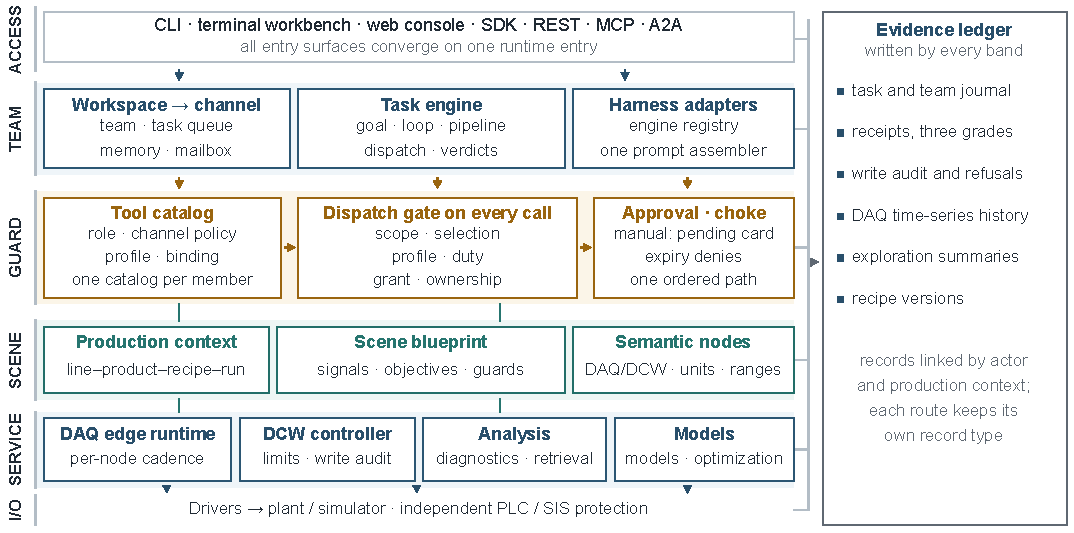
\includegraphics[width=\textwidth]{resources/fig-architecture-2026.pdf}
\caption{AgentWorkShop software architecture. Access, collaboration,
governance, production context, services, and field I/O form six connected
bands. Registered harness and driver interfaces expose extension points;
the evidence ledger retains route-specific records across the bands. The field
interface ends at the registered drivers; PLC and safety-instrumented
protection remain external.}
\label{fig:arch}
\end{figure*}
\section{System Design}
\label{sec:design}
AgentWorkShop is designed for industrial tasks whose agents, production
contexts, interfaces, and process signals vary between deployments. A useful
framework must let these differences be configured without changing the
shared task runtime, while ensuring that a proposed operation is checked
against the active production context before it reaches a device. It must also
retain enough route-specific evidence to distinguish a returned command
receipt from a measured process response.

\subsection{Design Rationale and Requirements}
\label{sec:principles}
The five requirements---scene variability, harness variability, operation
authority, observability, and extensibility---organize six design rules
(D1--D6). They are deployment constraints selected from the target workflows,
not a taxonomy inferred from a systematic review or an empirical coding study:
encode scene settings as versioned data; extend the runtime through registered
harness, tool, and driver interfaces; separate proposal from execution; treat
the tool catalog as discovery rather than permission; route actuator writes
through the common DCW admission point; and retain evidence by operation.
D1 maps to blueprints and context resolution; D2 to the harness, tool, and
driver registries; D3--D5 to task dispatch, binding/grant checks, and DCW
write admission; and D6 to route handlers and the evidence ledger. The
evaluation maps these rules to complementary evidence: Q1 and Q4 exercise
historical direct-node scene mappings; Q2 exercises two tasks with one
registered OMP harness; Q5 checks dispatcher and write-confirmation regressions
on v0.7.57; Q6 and the October 23 boundary record exercise recipe and approval
paths; and Q7 checks current v0.8.0 protocol acquisition, bounded writes,
readback, and data lineage across two simulator scenes. Q7 does not traverse
the registered harness or demonstrate profile adaptation, and these evidence
units do not form one end-to-end deployment trial. The results state available
version and interface provenance and identify gaps, including the unavailable
R1 runtime worktree and R6 commit. AgentWorkShop does not select an agent's
control strategy or replace independent controller and safety functions.

\subsection{Layered Architecture}
\label{sec:layers}
\label{sec:arch}
Fig.~\ref{fig:arch} maps the reference implementation onto six bands and a
shared evidence ledger. The access band exposes command-line, web, SDK, REST,
MCP, and A2A entry surfaces. The collaboration band contains workspaces,
channels, task queues, shared memory, mailboxes, task templates, and
harness adapters. The governance band projects an operation catalog and
checks each invocation. The context band binds a scene blueprint to the
active line--product--recipe--run tuple and its semantic DAQ/DCW nodes. The
service band provides acquisition, write control, analysis, retrieval, and
optional model services. The field-I/O band resolves semantic nodes to
built-in or plugin drivers for a plant or simulator.

Each band has a distinct responsibility. Entry surfaces converge on the
same task runtime; a harness adapter supplies the agent-specific interaction;
semantic nodes hide protocol details from the task; and the driver registry
provides the device-facing extension point. The evidence ledger records
task, command, observation, and version events against their actor and
production context. It does not collapse them into a single success flag.

\subsection{Cross-Module Execution Flow}
\label{sec:executionflow}
Fig.~\ref{fig:runtime} summarizes a task turn from entry to returned
evidence. The runtime resolves the production context and assembles the
prompt and scoped tool catalog before invoking a registered harness. For
each returned tool call, the shared dispatcher rechecks invocation scope
and channel policy; industrial operations also receive current grant and
binding checks before handler selection. The selected handler applies its
own route-specific guards, approval, revalidation, and device-I/O steps.
Command receipts and any later process observations remain distinct records.

Fig.~\ref{fig:execution} gives pseudocode for these cross-module contracts;
it is a reference flow rather than one literal orchestrator function.
Route-specific timing, approval, and evidence rules are detailed in
Section~\ref{sec:modules}.

\begin{figure*}[!t]
\centering
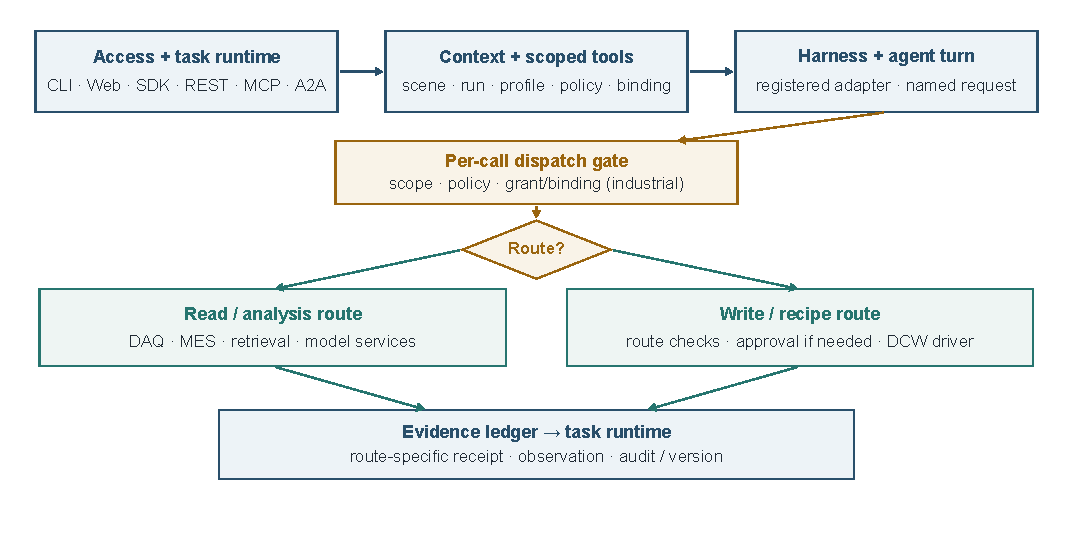
\includegraphics[width=\textwidth]{resources/fig-runtime-2026.pdf}
\caption{Cross-module task execution in AgentWorkShop. Entry and task
services assemble the channel-scoped tool catalog before the agent turn;
each returned call is rechecked for scope and policy, with grant and binding
checks for industrial operations. Dispatch-gate refusals stop before handler
execution, whereas route-specific handlers may read state before refusing a
write. Receipts and later observations remain distinct.}
\label{fig:runtime}
\end{figure*}

\begin{figure}[!t]
\centering
\begin{algorithmic}[1]
\Require task $q$, channel $c$, bound agent $a$
\Ensure task result and route-linked evidence
\State $x \gets \Call{ResolveContext}{c,q}$
\State $T \gets \Call{FilterToolCatalog}{a,c}$
\State $m \gets \Call{RetrieveMemory}{q}$
\State $p \gets \Call{AssemblePrompt}{q,x,m}$
\State $h \gets \Call{InvokeRegisteredHarness}{a,p,T}$
\ForAll{tool request $u$ returned by $h$}
  \State $g \gets \Call{CheckScopeAndChannelPolicy}{a,c,u}$
  \If{\textbf{not} $g$}
    \State \Call{RecordDispatchRefusal}{u,x}; \textbf{continue}
  \EndIf
  \If{$u$ is an industrial operation}
    \State $v \gets \Call{CheckGrantAndBinding}{a,u}$
    \If{\textbf{not} $v$}
      \State \Call{RecordDispatchRefusal}{u,x}; \textbf{continue}
    \EndIf
  \EndIf
  \State $k \gets \Call{SelectHandler}{u}$
  \State $r \gets \Call{ExecuteRouteHandler}{k,u,x}$
  \State \Call{RecordAvailableEvidence}{u,r,x}
  \State \Call{ReturnToolResult}{h,r}
\EndFor
\State \Return task state and retained evidence
\end{algorithmic}
\caption{Reference pseudocode for cross-module execution in AgentWorkShop.}
\label{fig:execution}
\end{figure}

\section{Module Functions and Integration}
\label{sec:modules}
The architecture in Fig.~\ref{fig:arch} is implemented as cooperating
modules rather than a single monolithic agent. Shared interfaces connect
task execution to configuration, industrial services, protocol drivers, and
route-specific evidence. This section describes those responsibilities and
the checks that preserve their boundaries.

The extension contracts expose the data passed at each boundary. A harness
call is normalized as \texttt{HostToolCall(toolName, arguments)} and returns
\texttt{HostToolResult(text, isError)}. A DCW driver accepts an engineering
value, tolerance, range, and driver configuration; its result separates write
status, raw value, readback, and acknowledgment grade (readback-verified,
transport-ack, or unverified). Each DAQ sample stores its node, timestamp,
value, and state, with optional line, product, recipe, and run IDs. A write
anchor records line/node, prior and requested values, source, actor, time, and
optional run/task/approval IDs; recipe definitions retain separate versions.
These fields keep tool errors, device receipts, observations, and production
lineage inspectable as separate records.

\subsection{Task Runtime and Harness Adapters}
An access surface creates or joins a workspace channel, where the task
engine manages members, task queues, shared memory, and execution templates.
The harness registry instantiates an adapter behind a common agent interface;
the prompt builder combines the task with the active scene brief, industrial
context, channel profile, agent binding, and retrieved memory. Tool calls
return to the shared dispatcher regardless of which registered harness
produced them. The registry is an extension point; the experiments do not
establish portability across harnesses.

\subsection{Production Context and Configuration}
Scene blueprints describe devices, signal maps, objectives, and process
guards. A task resolves these definitions against its active
line--product--recipe--run context. The channel profile selects the available
capability family, the tool policy narrows the operation catalog, and the
agent binding scopes the nodes, controls, and recipe operations available to
that member. These filters can restrict one another but cannot broaden the
underlying device range. The dispatcher re-reads policy at execution, so a
cached catalog does not retain authority after a grant or policy change.

\subsection{Acquisition, Analysis, and Modeling Services}
Semantic DAQ nodes expose typed values, engineering units, ranges, and
sampling settings while hiding protocol-specific reads. A per-node DAQ
runtime schedules acquisition and stores timestamped observations; the
gateway aggregates node pipelines. MES-facing operations provide the
configured production-data path. Analysis and retrieval services consume
these records, while optional model, training, optimization, and digital-twin
services are invoked through their registered operation handlers. These
services complement the agent workflow; AgentWorkShop does not prescribe a
single optimization strategy.

\subsection{Semantic I/O and Actuation}
The driver registry resolves a semantic node to a built-in or plugin driver.
DAQ handlers use the node's acquisition interface; DCW handlers route a
write or readback through the controller and the configured protocol driver.
This separation lets recipes and agents refer to semantic controls without
embedding Modbus, OPC UA, MQTT, HTTP, or MES transport details in their
operation arguments. The supported driver mappings are implementation
interfaces; only the mappings and workflows enumerated in Section~\ref{sec:eval}
are experimentally exercised.

\subsection{Shared Dispatch and Write Admission}
\label{sec:governed}
Every named operation passes the dispatcher. Its ordered checks validate
invocation scope, channel tool selection, profile, duty separation, the
agent's binding and runtime grant, and ownership of referenced resources.
A refusal returns the excluding condition and is recorded. A catalog entry
therefore describes availability but does not authorize execution. Handlers
for operations that require manual approval suspend for a decision, then
revalidate authority and active limits before dispatch.

All actuator writes converge on the DCW admission point. For an online node
write, the admissible interval is
\begin{equation}
\mathcal{I}^{\mathrm{online}}_n(t)=\mathcal{H}_n\cap\mathcal{B}_n
\cap\mathcal{P}_n(t)\cap\mathcal{R}_n(t),
\label{eq:admission}
\end{equation}
where $\mathcal{H}_n$ is the hard engineering range and $\mathcal{B}_n$,
$\mathcal{P}_n$, and $\mathcal{R}_n$ are the baseline, active-product, and
active-recipe limits. Missing optional limits impose no restriction, whereas
an empty intersection rejects the request and identifies the excluding
layer. Recipe dispatch applies the hard, baseline, and product limits to the
replacement recipe rather than intersecting with the previous recipe window.
The actuator path also enforces step, interval, and hold-window checks.
These admission rules constrain commands; process objectives and coupled
variable guards are assessed from later observations. The framework does
not replace independent PLC or safety-instrumented protection.

\subsection{Integrated Operation and Route-Specific Evidence}
\label{sec:tasklifecycle}
A recipe trial illustrates how the modules cooperate. The task runtime
delivers a named \texttt{recipe\_trial} call from the agent harness; the
dispatcher checks the agent's recipe binding and execution scope; the recipe
handler checks the active run, candidate parameters, and route timing; and a
manual binding requests approval before the DCW controller sends the batch
through its driver. The handler returns a per-parameter receipt. The caller
then obtains DAQ observations and can request a separate update, apply, or
rollback operation. A trial receipt confirms command handling; it does not
by itself establish process attainment or persist a new recipe version.

The routes retain different records because they answer different
questions. A driver acknowledgment reports command evidence; DAQ reports a
process observation; an exploration summary records a bounded probe; and a
recipe version records a saved definition. Their relation through actor and
production context allows an execution to be inspected without treating
these outcomes as interchangeable.

\subsection{Route-Specific Lifecycles and Evidence}
\label{sec:routes}
\label{sec:mech}
\label{sec:objective}
\label{sec:nodeexec}
\label{sec:ack}

\paragraph{Timing and approval}
Timing guards are route-specific. Online node writes enforce an effective
minimum spacing of 60\,s. Recipe dispatch uses a per-recipe interval anchored
to approval, while trials also use a configurable per-line cadence (default
300\,s). The recipe interval can refuse a proposal before an approval request
is created. Checks occur at proposal or execution according to the operation,
and experiment-specific pacing overrides are reported with the corresponding
results.

Manual bindings create an approval request containing the actor, node or
recipe, candidate values, applicable limits, expiry, and parameter bases.
The default wait expires after 180\,s and refuses execution. After approval,
the executor rechecks authorization and active limits to account for context
changes during the wait. For \texttt{recipe\_apply}, a changed definition
requires a new proposal; an unchanged approval dispatches a copy of the
approved parameter snapshot. A line-level recipe mode defaults to manual;
changing it to automatic requires administrator confirmation. The approval
record authorizes a workflow action and does not replace process protection.

\begin{figure*}[!t]
\centering
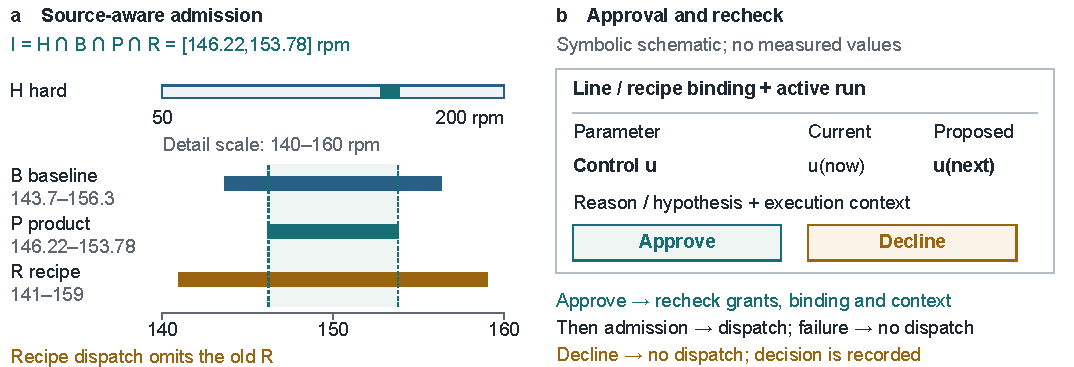
\includegraphics[width=\textwidth]{resources/fig-admission-hitl-2026.pdf}
\caption{Admission and approval boundaries. (a) Archived Q1 RPM example:
online node interventions use the four-layer value interval of Eq.~(1),
whereas recipe dispatch omits the prior recipe window. (b) Symbolic human
approval binds a proposed action and authority fields; execution checks run
again after approval, which does not reserve equipment state.}
\label{fig:hitl}
\end{figure*}

\paragraph{Node probe}
The bounded node probe is exposed as \texttt{optimization\_explore} to the
Auto Modeling Lab (AML) optimization profile (\texttt{aml\_optimization}).
The profile validates a bound control and target DAQ scope,
captures a starting control and target baseline, invokes the internal DCW
write path, then waits 10--300\,s (default 45\,s) and queries a trailing 45-s
target window before saving an exploration summary. Since each window is
relative to its query time, approval can separate baseline sampling from
actuation; a 10-s wait can leave about 35\,s of pre-write samples in the later
window. The command receipt and target summary are therefore returned
separately. A successful changed-value write opens a node-optimization
record; refusal or expired approval creates a rejected summary without a
post-write sample.

\paragraph{Recipe operations}
\texttt{recipe\_trial} checks the bound recipe and active run, then dispatches
candidate overrides as a batch with per-parameter verification. The caller
subsequently queries DAQ and decides whether to save a new definition with
\texttt{recipe\_update}, restore one with \texttt{recipe\_rollback}, or
dispatch a version with \texttt{recipe\_apply}. These steps are separate: a
trial does not save or apply a version, and endpoint verification is not a
process-response measurement. Public direct-node control is closed; the
bounded probe and recipe operations are the configured operation surfaces.
The historical four-scene results use an earlier direct-node path and do not
test current profile or binding adaptation across scenes.

\paragraph{Command verification}
Command confirmation and process response answer different questions. A
driver ACK is graded as \texttt{readback-verified}, \texttt{transport-ack},
or \texttt{unverified}. A matching endpoint read supports the first grade; a
transport or MES application receipt supports the second. Recipe batch
verification assigns \texttt{verified}, \texttt{unverified}, or
\texttt{failed}; if no matching readback is available, it attempts up to
three independent reads, 2\,s apart. A matching retry upgrades the final ACK,
while exhausted retries remain unverified. The initial ACK remains in write
history and the final ACK and verdict are retained with the batch.
Per-parameter receipts preserve successful outcomes when another parameter
fails. A readback-verified setpoint does not establish target attainment.

\paragraph{Observation, verdict, and compensation}
The caller performs recipe-path observation after batch dispatch. The October
recipe case therefore compares a recipe definition, endpoint readback, and
DAQ sample as separate representations. Saving a definition, applying it to
equipment, and observing its process response are separately evidenced
operations. The evaluation does not combine these route-specific records into
one universal end-to-end record.

An open node record provides a monitoring backstop. After 120\,s it polls
every 30\,s; three cumulative samples outside the recipe monitoring window
trigger a system-attributed rollback request toward the preceding value.
Missing samples do not count as breaches. A caller's \texttt{keep},
\texttt{rollback}, or \texttt{uncertain} verdict records its interpretation;
compensation is a new command subject to its applicable admission policy.
The write audit deduplicates the same value on the same node within 10\,s,
while batch receipts, exploration summaries, DAQ history, and recipe versions
retain their distinct lifecycles. Linking these records by actor and
production context allows the command, endpoint evidence, and process
observation to be inspected without treating them as interchangeable.
\label{sec:agentloop}


\FloatBarrier
\section{Experimental Evaluation}
\label{sec:eval}
The evaluation asks whether the framework connects configured process scenes
through the current software stack, and what the archived process, protocol,
and route-level evidence establishes beyond that integration check. It combines
a current-version two-scene simulator run with historical process trajectories,
protocol exercises, live-engine tasks, a deterministic controller,
deployment regressions, and a recipe case. These evidence units are not
matched trials or a paired strategy comparison. Q1--Q6 retain their historical
archive identifiers; Q7 denotes the current-version integration run. These
labels identify evidence groups rather than posed research questions. All
process experiments use repository simulators. The reproducibility notes map
each claim to its source and interface version.

\subsection{Evidence Units and Experimental Procedure}
\label{sec:testbed}
\label{sec:procedure}
Q1--Q4 use the seed-\resSeed{} integrated archive (R1) and its raw scenario
records; the admission ablation uses a separate companion run (R2). R1 can
be audited, but its historical runtime worktree is not archived, so the
recorded source commit does not guarantee exact replay. These historical
missions use the direct-node interface and scripted proposal policies,
apart from the two Q2 live-engine tasks. Q3 additionally uses seeds 43--44;
Q5 uses nine deployment-suite executions, and Q6 uses the October 18 recipe
archive. The cast-film reference preset uses an author-defined objective $J$
combining thickness conformance, defects, energy, and throughput.

The same 65 profile/composition checks passed on October 20, 24, and 25 with
temporary storage and mock I/O; these repeated software checks are not 195
independent assertions or process trials. Q4 retains one seed-42 trajectory
per scene, with sequential writes and post-wait observations.

Q5 covers 20 deployment phases in nine historical v0.7.57 runs; its 782
assertions are software checks, not current-version or plant results. Six
writes per protocol line yield an upper median and observed maximum, not a
tail percentile.

\subsection{Current-Version Two-Scene Simulator Integration (Q7)}
\label{sec:crossscene}
An isolated local v0.8.0 application ran the cast-film and annealing simulator
presets. The five configured protocol-driver families---OPC UA, MQTT,
Modbus TCP, Modbus RTU over TCP, and HTTP/REST---passed read probes, and
scene-specific DCW writes returned matching readbacks. Six 120-s runs per
scene at 1-s sampling yielded lineage-verified datasets (Table~\ref{tab:q7});
neither the simulator truth/optimum endpoint nor an external LLM service was
used.

Eligibility used paired row values: MV at the end of the history window and
CV at the start of the forecast horizon. After first differences, the service
selected the signed Pearson correlation between $\Delta$MV and lagged $\Delta$CV
with greatest absolute magnitude over row lags 1--3.
This configured gate tests only that three-row window; a failed pair does not
establish the absence of a delayed physical response outside it.

This differenced-series gate statistic is distinct from the
dataset builder's descriptive raw-level correlation from the first training
run over $\pm20$ lags (see \path{REPRODUCIBILITY.md}). The configured gates
required $|r_{\Delta}|\geq0.2$, one-step test normalized root-mean-square error
(NRMSE) $\leq0.10$, and at least a 20\% reduction in four-step rollout NRMSE
relative to persistence, defined as $1-\mathrm{NRMSE}_{\mathrm{rollout}}/
\mathrm{NRMSE}_{\mathrm{persistence}}$. Both candidates were rejected, with
no profile, recommendation, or dispatch. Each test split used two of the six
120-s runs (220 film rows and 218 annealing rows); the overlapping 1-s windows
are serially dependent, not independent trials. The reported signal
pairs followed an exploratory pilot and inspection of preset mappings; both
pilot models also failed. Q7 therefore demonstrates the current protocol/data
path and gate behavior, not a current registered-harness process intervention
or confirmatory model performance. The pilot and final-run data are retained
separately in the evidence supplement.

\begin{table*}[!t]
\centering
\caption{Current v0.8.0 two-scene simulator integration (one dataset per
scene; six sequential 120-s runs per dataset). Counts are DAQ points, dataset
rows, and held-out test rows. Each test split uses two runs per scene;
overlapping 1-s rows are serially dependent, not independent replicates.}
\label{tab:q7}
\small
\setlength{\tabcolsep}{4pt}
\begin{tabularx}{\textwidth}{@{}l X >{\centering\arraybackslash}p{2.3cm} X@{}}
\toprule
Scene & Manipulated and controlled signals & DAQ points / rows / test rows & Eligibility and held-out result \\
\midrule
Cast film & Screw speed (OPC UA) $\rightarrow$ thickness (MQTT) & 697 / 658 / 220 & Blocked; $|r_{\Delta}|=0.095$ (lag 2 rows), one-step NRMSE $=0.259$, four-step reduction $=14.1\%$ \\
Annealing & Zone-3 temperature setpoint (Modbus TCP) $\rightarrow$ strip temperature (Modbus TCP) & 696 / 655 / 218 & Blocked; $|r_{\Delta}|=0.053$ (lag 3 rows), one-step NRMSE $=0.363$, four-step reduction $=4.8\%$ \\
\bottomrule
\end{tabularx}
\end{table*}

\subsection{Historical Four-Process Simulator Missions (Q4)}
\label{sec:scenarios}
The concurrent campaign provides one seed-42 trajectory per process.
Figure~\ref{fig:missions} pairs archived manipulated controls $u$ with the
corresponding response $y$ rather than showing response alone. All four
terminal attainment checks passed; two lay near a target boundary.

Injection molding used two changes: hold pressure
$45\rightarrow58.2$\,bar and hold time $6\rightarrow10.64$\,s. Part weight
rose from \resInjStart{} to \resInjFinal{}\,g for a
$32.5\pm0.35$\,g window, only $0.02$\,g above its lower limit.
Biaxially oriented polyethylene terephthalate (BOPET) changed casting speed
$32\rightarrow33.8$\,m/min, fast-roll speed
$118\rightarrow120.3$\,m/min, and rail width $3000\rightarrow3035$\,mm.
Thickness fell from \resBiaxStart{} to \resBiaxFinal{}\,$\mu$m for a
$25.0\pm0.7$\,$\mu$m target, $0.04$\,$\mu$m inside the upper limit.
Its three changes each have a recorded keep verdict and journal identifier.

Wastewater treatment required 15 writes across several nodes. Dissolved
oxygen rose from \resWwtpStart{} to \resWwtpFinal{}\,mg/L, within
$3.4\pm0.6$\,mg/L. Some admissible blower proposals reduced compliance
margin and were reverted. Terminal guards remained within their declared
limits, although pH moved toward its lower bound (6.59 to 6.38; limit 6.0).
Dissolved oxygen, total phosphorus (TP), and pH are different quantities
and are not concatenated into one output trajectory.

Annealing combined furnace-temperature changes with line-speed increases
from 140 to 164\,m/min. The recorded Vickers hardness (HV) trajectory moved from
\resAnnealStart{} to 99.84\,HV; the separate terminal measurement was
\resAnnealFinal{}\,HV, within $95\pm6$\,HV. A 176\,m/min attempt produced
101.3\,HV and was reverted. The first temperature step has no optimization
record identifier in the archive, which bounds record-level traceability.
These historical missions document process behavior under a shared scripted
task scaffold and retain the distinction between a candidate command, a
reverted candidate, and a terminal observation. They do not evaluate
current profile or per-agent binding variation across scenes.

\begin{figure*}[!t]
\centering
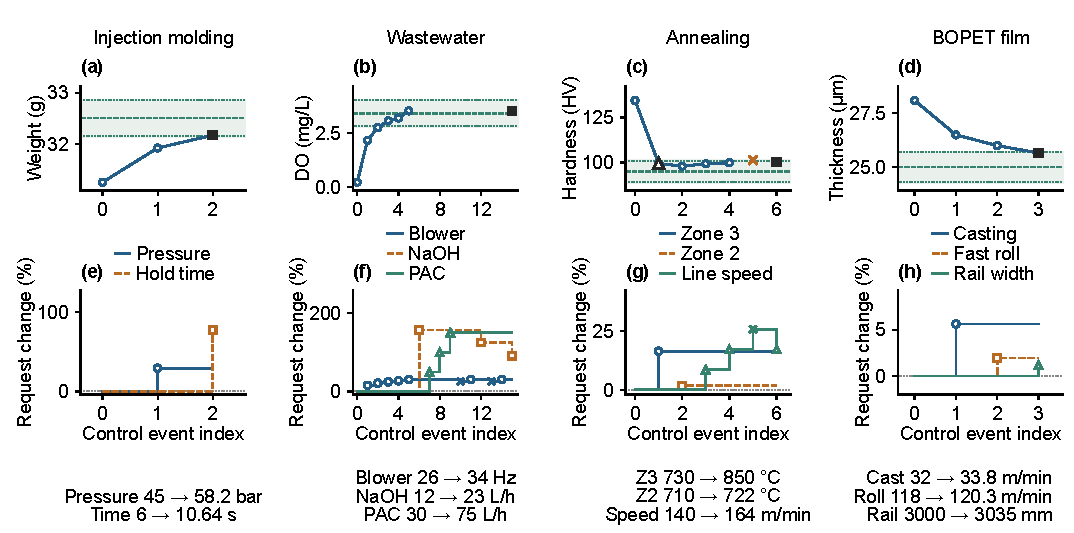
\includegraphics[width=\textwidth]{resources/fig-missions-controls.pdf}
\caption{Historical scripted missions (seed 42, one trajectory per process).
(a--d) Weight, dissolved oxygen (DO), hardness, and film thickness with their
target windows. (e--h) Requested controls as percentage change from native
baselines: injection pressure 45\,bar/time 6\,s; wastewater blower
26\,Hz/NaOH 12\,L/h/PAC 30\,L/h; annealing zone 3
730$^{\circ}$C/zone 2 710$^{\circ}$C/speed 140\,m/min; BOPET casting
32\,m/min/fast roll 118\,m/min/rail 3000\,mm. Lines connect event indices,
not physical time; unchanged requested values carry forward. Crosses mark
reverted candidates and squares distinct terminal observations. The open
triangle in panel (c) marks the first annealing observation, which lacks an
optimization-record ID. DO excludes pH/TP events.}
\label{fig:missions}
\end{figure*}

\subsection{Heterogeneous Protocol Integration and Route Checks (Q1)}
\label{sec:protocol}
The suite acquired \resDaqSamples{} samples over five protocol families and
issued policy-checked writes over four; the RTU-over-TCP line was
acquisition-only.
Archived upper-median write latencies ranged from \resPfiftyRange{}, with observed maxima
\resPninetyfiveRange{}. The four writable lines accepted legal writes and
rejected 24/24 out-of-window probes. A configuration-only second preset
added 9/9 rejected probes on three further writable lines. These results
exercise the same resolver against different signal maps.

In a mock-driver API fixture, three deterministic repetitions of six attack
classes per arm isolated admission from endpoint confirmation. With the
soft-window interlock enabled, both the full and no-readback arms refused
all 18 attacks. Disabling the interlock allowed the six soft-window probes
to execute, while the 12 hard-range probes remained refused. Removing
readback did not change admission, showing that confirmation cannot replace
a pre-write gate. A frozen-measurement drill further separated command and
process evidence: the setpoint and readback agreed, yet the monitoring
quantity remained outside its window and triggered backstop rollback after
\resBackstop{}. A manual-binding drill suspended execution until
harness-issued approval (\resHitlLatency{} mediation span).

\subsection{Live-Engine Tasks and Deterministic Controller (Q2--Q3)}
\label{sec:agentteam}
The archived team workflow linked a parent task, a bound worker, a command,
a verdict, and its journal. On the single-node cast-film mission, the policy
changed the heater from \resMissionFrom{} to
\resMissionTo\,$^{\circ}$C; the observation settled at
\resMissionPv\,$^{\circ}$C within the declared target. The task reached
\texttt{COMPLETED}. The BOPET mission expanded this workflow to nine devices
and 49 signals, with three manipulated nodes
(Section~\ref{sec:scenarios}).

Two live-engine tasks used the same \texttt{omp} harness, Zhipu Coding Plan
provider, and GLM-5.3-Flash model on a scratch line; they are execution
traces, not a strategy comparison or a cross-harness portability test. The archive
records a bounded write, a goal-driven
descent to \resGoalFinal\,$\mu$m for a $52.0\pm0.8$\,$\mu$m target, and a
recipe save. The original contemporaneous omp logs and checked run outcomes
trace proposal, policy-checked action, observations, and retained recipe.
The reported \resGoalFinal\,$\mu$m is the run-summary terminal value;
the log's 52.02\,$\mu$m window mean is a different aggregation.

\label{sec:controller}
A deterministic controller used the dimensionless cast-film objective
\begin{equation}
\begin{aligned}
J={}&55J_{\mathrm{thick}}+25J_{\mathrm{quality}}\\
&+8J_{\mathrm{energy}}+7J_{\mathrm{throughput}},
\end{aligned}
\label{eq:objective}
\end{equation}
whose components score thickness conformance, product quality, and
control-based energy and throughput proxies. The latter two terms use
screw speed and line speed, rather than independently metered energy and
production output. This deterministic-controller experiment is not an
evaluation of AgentWorkShop's optional model service. Table~\ref{tab:q3search}
summarizes its finite candidate grid and selection rule; component formulas
and replay details are provided in \path{REPRODUCIBILITY.md}.

\begin{table*}[!t]
\centering
\caption{Finite-grid search protocol for the deterministic cast-film
controller in Q3. The reference score is restricted to this grid and is not
a global continuous optimum.}
\label{tab:q3search}
\footnotesize
\setlength{\tabcolsep}{4pt}
\begin{tabularx}{\textwidth}{@{}p{2.4cm}Xp{3.0cm}@{}}
\toprule
Search element & Candidate set or rule & Role in the search \\
\midrule
Objective & Eq.~(\ref{eq:objective}); weights 55/25/8/7 for thickness,
quality, energy proxy, and throughput proxy & Rank eligible steady states \\
Eligibility & Melt temperature 195--225~$^{\circ}$C; melt pressure
$\leq 22$~MPa & Discard ineligible states \\
Equal zone setpoint & 195--225~$^{\circ}$C in 2.5~$^{\circ}$C steps & Search variable \\
Screw speed & 50--200~rpm in 5-rpm steps & Search variable \\
Line speed & 20--120~m/min in 2.5-m/min steps & Search variable \\
Die gap & Fixed at 1~mm & Held constant \\
Selection & Evaluate modeled steady state and retain the highest eligible
score; $J^{*}=89.894$ & Finite-grid reference \\
\bottomrule
\end{tabularx}
\end{table*}

Across seeds 42--44, this single controller made two policy-checked writes per
seed, without rejection. It raised $J$ from approximately
\resJzero{} to $J/J^*=\resControllerMin$--\resControllerMax{}, with
$J^*=\resJstar$ from the admissible setpoint grid. This reference
normalization is restricted to the finite search space.
The result links the controller's native objective to admissible commands
and endpoint evidence, exercising a conventional strategy through the
same execution services.

\subsection{Deployment Composition and Confirmation Semantics (Q5)}
\label{sec:hardening}
The deployment suite composed \resLinesLive{} lines, \resChannelsLive{}
channels, \resDaqOnline{} online DAQ nodes, \resWriteNodesLive{} write nodes,
\resRecipesLive{} recipes, and \resBindingsLive{} bindings on one simulator
host. Its injection workflow exercised proposal, pacing, approval, batch
dispatch, and recipe/readback/mirror comparison. The recorded sources agreed
within their tolerances (maximum deviation \resConsistencyErr{}), confirming
setpoint consistency but not process convergence. S4 remained
\texttt{converged=false}; observation-to-verification at 65\,bar took
96.105\,s. S5 applied 40-to-40.5$^{\circ}$C, refused the next write, and
restored 40$^{\circ}$C after a 66.046\,s wait. These are server/harness spans; approval-to-dispatch spans
were \resHitlDispatchMs{}.

Seven injected fault tests checked receipt grading: a mock acceptance needed
reread, a broker outage failed one parameter while its sibling verified, and
a publish-only endpoint remained unverified despite its broker receipt.
Additional checks covered readback promotion and manual-mode confirmation.
MES application receipts were covered by route tests; the deployment run used
MES only for reads. These outcomes characterize the tested fault conditions,
not real-world fault rates.

\subsection{Operational Recipe Workflow Case Study (Q6)}
\label{sec:recipeexperiment}
R6 is one October 18 injection-simulator trajectory, replayed through OPC UA
setpoints and HTTP quality acquisition. Its source commit, seed, and
per-sensor timestamps are unavailable; a live agent diagnosed insufficient
packing, but the intervention and approvals were scripted. From 45\,bar with
6-s hold time, four approved 5-bar \texttt{recipe\_trial}s each waited 65 s
before a DAQ check. The run saved recipe version 2 but did not apply it.
Table~\ref{tab:q6actions} records the sequence.

\begin{table*}[!b]
\centering
\caption{Recorded Q6 injection-recipe actions and post-wait observations
($n=1$ simulator trajectory). Hold time remained 6\,s; each trial used
harness approval, a 65-s wait, and a 1/1 parameter-verification receipt.}
\label{tab:q6actions}
\footnotesize
\setlength{\tabcolsep}{3.5pt}
\begin{tabularx}{\textwidth}{@{}l c c c c X@{}}
\toprule
Stage & Pressure (bar) & Weight (g) & Flash (\%) & Sink (\%) & Recorded action and outcome \\
\midrule
Baseline & 45 & 31.28 & 0 & 1.977 & No command; initial observation \\
Trial 1 & 45$\rightarrow$50 & 31.49 & 0.014 & 1.956 & Approved; 1/1 verified; continue \\
Trial 2 & 50$\rightarrow$55 & 31.74 & 0.031 & 1.760 & Approved; 1/1 verified; continue \\
Trial 3 & 55$\rightarrow$60 & 32.05 & 0 & 1.534 & Weight below 32.15-g minimum and sink above 1.50\%; continue \\
Trial 4 & 60$\rightarrow$65 & 32.30 & 0.019 & 1.277 & Stop recorded; displayed values are within ranges \\
Save & 65 & --- & --- & --- & \texttt{recipe\_update} saved version 2; no \texttt{recipe\_apply} is archived \\
\bottomrule
\end{tabularx}
\end{table*}

R6 disabled per-line trial cadence and bypassed the separate recipe-operation
interval; approval, admission, and command confirmation remained active.
Melt temperature was missing, and the stop used only weight, flash, and sink
mark. The freshness check used the newest available timestamp, so it does not
prove simultaneous per-sensor freshness. We report the recorded stop with
displayed values in range, not an independently audited guard pass; the later
update rationale contains unlinked quality values. A separate 65-to-70\,bar
check began from another state and is not a replicate. In October 23 boundary
checks, the public route refused eight direct-node writes; the default-cadence
recipe route verified one trial, then refused later proposals and failed to
restore the 45-bar baseline (4/8 assertions passed). These are separate
failed boundary records, not repetitions of R6.

\FloatBarrier
\section{Discussion}
\label{sec:limits}
Q7 verifies current-version protocol integration and lineage-checked
acquisition in two simulator scenes, but both exploratory datasets fail the
model gates and do not establish transfer. Historical Q4 used a shared
scripted scaffold and direct-node interface; profile checks used mock I/O.
Current profile and per-agent-binding adaptation, and the registered-harness
path combined with Q7, remain untested.

Q6 saved but did not apply a recipe; its cadence-bypassed stop does not prove
simultaneous sensor freshness. A separate default-paced check missed its
target and failed restoration, so neither trace establishes recipe-recovery
readiness. Approval records do not measure operator effectiveness
\cite{parasuramanmanzey2010complacency,parasuraman2000model,bainbridge1983ironies};
restricted tool access does not establish deployment security
\cite{greshake2023injection,liu2024pinjection,iec62443-3-3} or replace
independently engineered PLC/SIS protection \cite{iec61511}.

Further evaluation needs a versioned build, matched scenes, a predeclared
signal-pair and excitation plan, and default-paced recipe baselines. Physical
plant tests are required to establish transfer beyond repository simulators.

\section{Conclusion}
\label{sec:conclusion}
AgentWorkShop integrates collaborative harnesses, production context, model
services, semantic I/O, and node/recipe workflows while retaining distinct
authorization, command-confirmation, and observation records. Historical
archives and the current two-scene run verify selected software paths, but
the current model gates withhold both recommendations. Successful
optimization, cross-scene transfer, cross-harness portability, recipe
recovery, plant transfer, and comparative control benefit remain unestablished.


% TII's anonymous-review checklist requires acknowledgments to be omitted.
% Restore the separate AI disclosure after the review stage; see the author note.

\bibliographystyle{IEEEtran}
% Keep IEEEtran's default bibliography size and leading.
\bibliography{resources/refs}

\end{document}
